\documentclass[10pt, letterpaper]{article}
\usepackage{graphicx}
\usepackage[bottom=1.0in]{geometry}
\topmargin=-0.9in
\oddsidemargin -.3in
\evensidemargin -0.3in
\textwidth=7.0in
%\itemsep= -0.5in
%\parsep= -0.04in

\usepackage[cmex10]{amsmath}
\usepackage{multirow}



\author{Madhusudan Govindraju 39267182 }
\date{}
\begin{document}
\title{EEL5840  Elements of Machine Intelligence - HW 5}
\maketitle

The document explains all the assumptions and the steps undertaken to complete the assignment and the results  are attached.

\begin{enumerate}
\item

\begin{enumerate}
\item The given feature set is 4 features per sample. Totally 150 samples.
\item \textbf{Case 1}:First the number of clusters are assumed to be 3 (K=3) and we choose  mean = 0 so the mean vector is $V_1 = [0,0,0,0]$ \& $V_2 = [0,0,0,0]$ \&$V_3  = [0,0,0,0]$
\item With this set of mean we calculate the membership matrix using the membership function shown in the figure \ref{fig:MembershipFunction}. Here the $||x_i - v_j|| =$euclidean distance between $x_i \& v_j$ and so on.

\begin{figure}[h!]
\centering
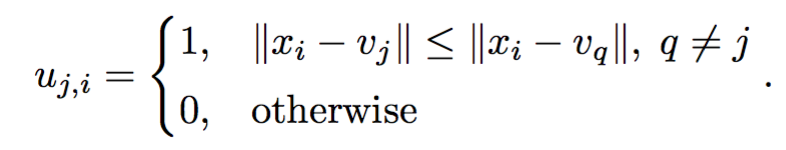
\includegraphics[scale = 0.5]{MembershipFunction}
\caption{Membership Function}
\label{fig:MembershipFunction}
\end{figure}

\begin{figure}[h!]
\centering
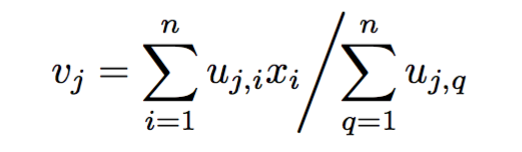
\includegraphics[scale=0.5]{UpdateMean}
\caption{ Update Mean Function}
\label {fig:UpdateMean}
\end{figure}

\begin{figure}[h!]
\centering
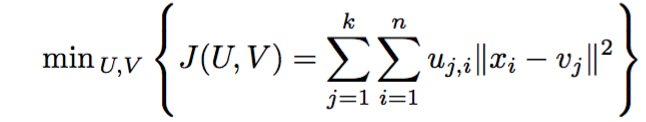
\includegraphics[scale=0.5]{ObjectiveFunction}
\caption{ Objective Function}
\label {fig:ObjectiveFunction}
\end{figure}





To calculate the distance between the sample and the mean 

To break ties in this step : If the sample is equidistant to two clusters 1 and 2, we label the sample under cluster 1.  and so on. So we choose sample to be in the first cluster among the group of clusters that are in a tie. So every sample will only be a part of one cluster.

\item After the membership matrix is populated with the membership function the cluster means are recalculated from the membership matrix. Using the formula in fig \ref{fig:UpdateMean}

\item With Membership Matrix and Mean calculated we can calculate {\sl J} with the formula in the figure \ref{fig:ObjectiveFunction}


\item repeat steps {\sl c} {\sl d} and {\sl e} until the mean does not change or the cost J does not change. 

\item The plot of J vs iterations is available in the fig \ref{fig:JvsI0}

 \begin{figure}[h!]
\centering
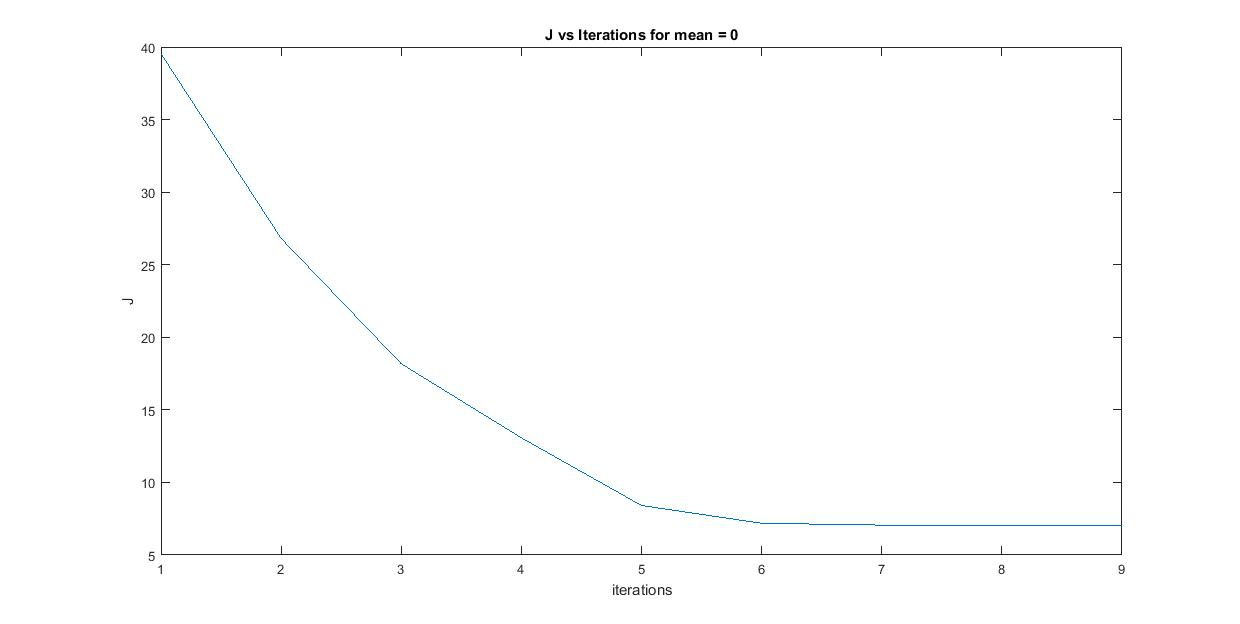
\includegraphics[scale=0.40]{JvsIterations_0mean}
\caption{J vs Iterations - For initial mean = 0 }
\label {fig:JvsI0}
\end{figure}

\begin{figure}[h!]
\centering
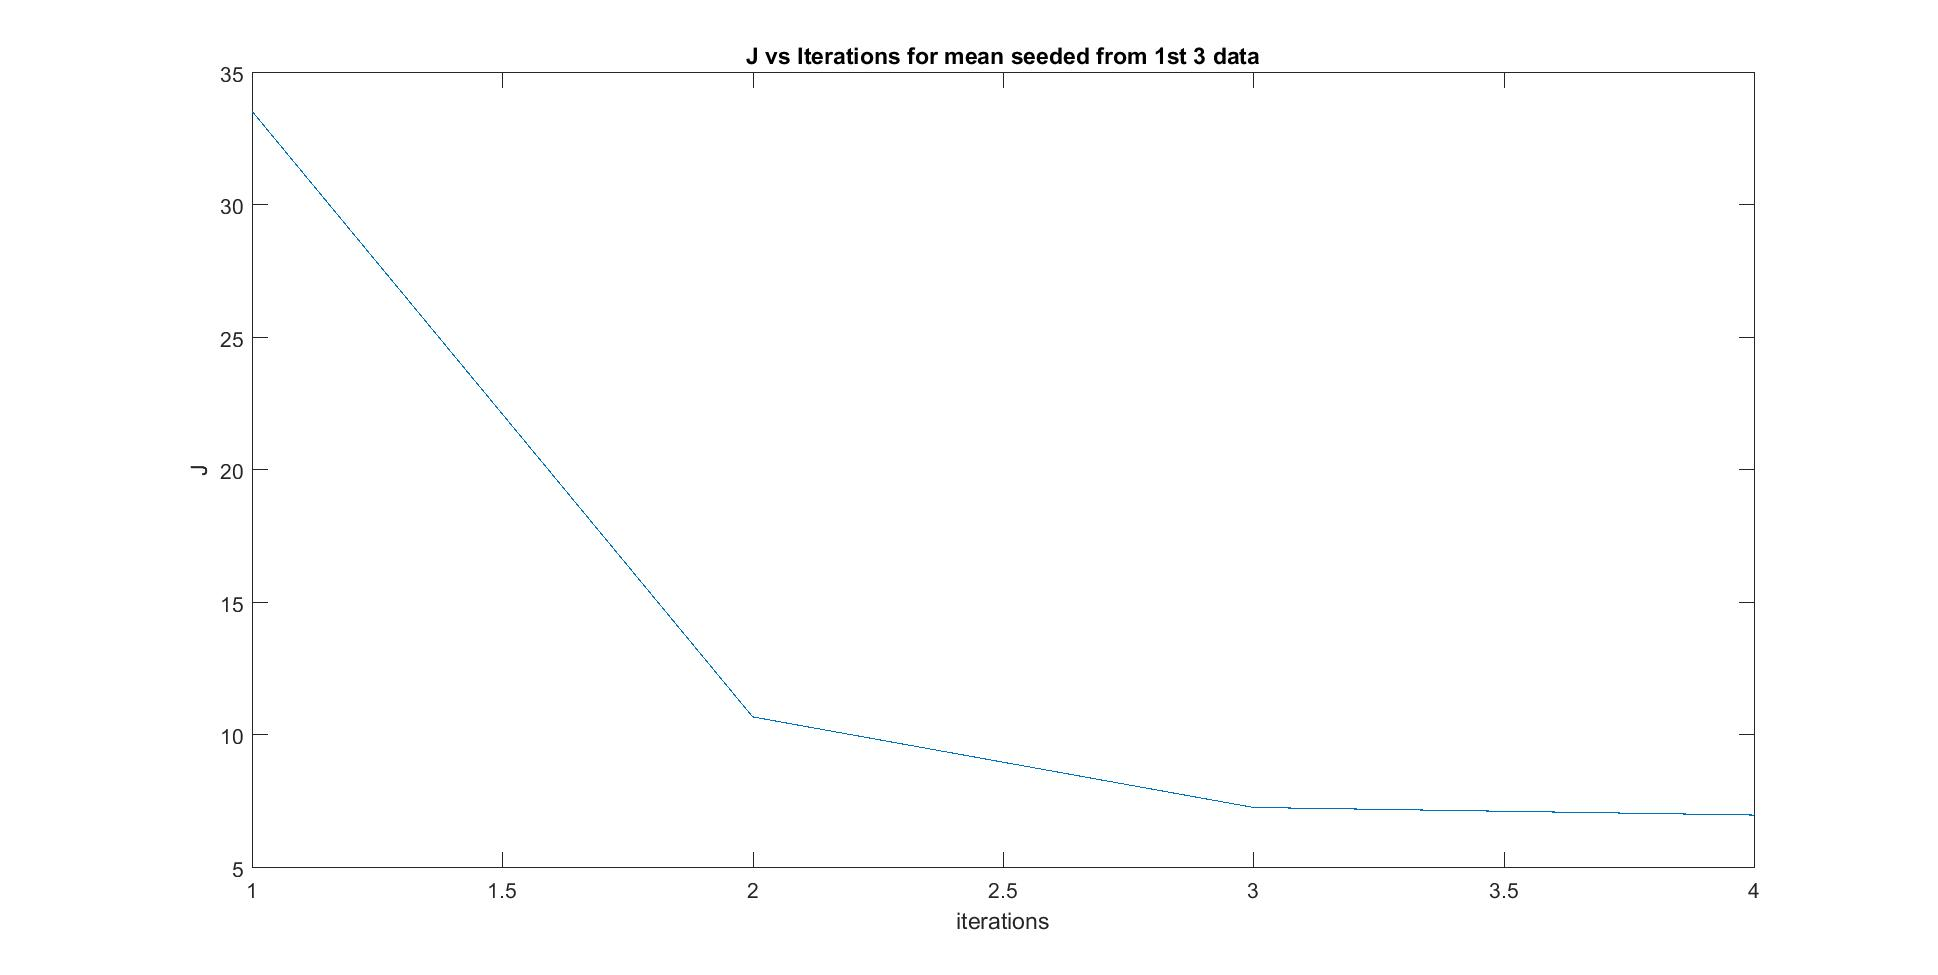
\includegraphics[scale=0.25]{JvsIterations_1mean}
\caption{J vs Iterations - For mean seeded from the dataset 1 }
\label {fig:JvsI1}
\end{figure}

 \begin{figure}[h!]
\centering
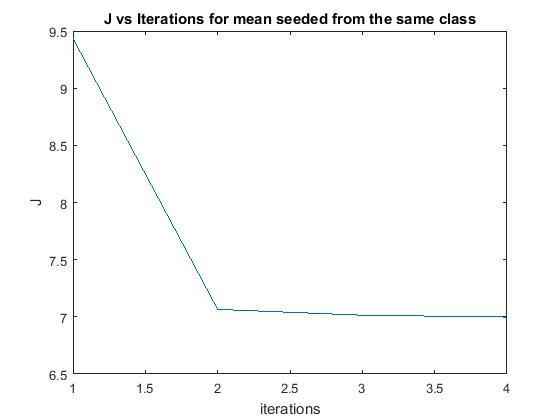
\includegraphics[scale=0.75]{JvsIterations_2mean}
\caption{J vs Iterations - For mean seeded from actual cluster }
\label {fig:JvsI2}
\end{figure}
 
 \begin{figure}[h!]
\centering
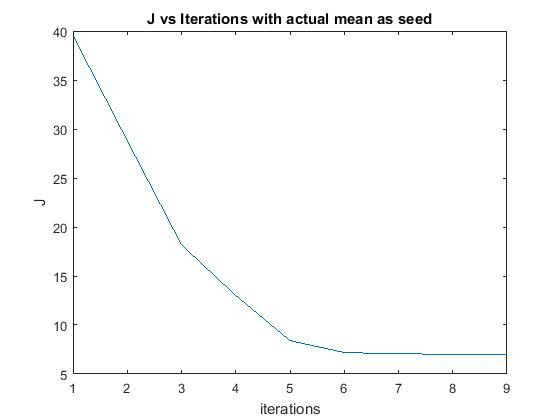
\includegraphics[scale=0.75]{JvsIterations_3mean}
\caption{J vs Iterations - Seeded with Actual Mean  }
\label {fig:JvsI3}
\end{figure}
 
\item Repeat the above steps for different values of means, by taking seed from the dataset.

\begin{enumerate}
\item \textbf{Case 2}: The seed is the first 3 samples from the dataset given. The plot of the cost vs the iterations is available in the fig \ref{fig:JvsI1}.  From this we can understand that the algorithm reaches the local minimum much sooner than when the mean was seeded with 0. Also a comment about the result is that, choosing this seed has resulted in a higher error rate which maybe because, the initial mean chosen was not in the the same space of the respective cluster( the seed for cluster2's mean  and cluster3's mean were taken from cluster 1; as we choose first 3 samples as mean for 3 classes)

 
\item \textbf{Case 3}: Now choose a data from the actual cluster to seed the respective cluster mean. The cost vs iterations graph for this case is available in the fig \ref{fig:JvsI2}. For this case we can see that the loop reaches the local minimum in just 4 iterations. Because we have seeded the mean from the data from the actual cluster the starting cost {\sl J } is much lesser compared to the other case. In the earlier cases it was around $35-40$. But in the current case the starting {\sl J} is only around 9.5.


\item \textbf{Case 4}: Now seed the means with the actual cluster means with information from the dataset. The number of iterations is 9. This case is similar to case 1. Also the error rate remains at the same value.

\end{enumerate}

\item \textbf{Observations} : From the above cases, we can understand two things, choosing the mean is important and the K means algorithm reaches the local minimum not the global minimum( understod from the result in the case 2). We should choose the mean from the actual sample space or start from 0. But starting from zero mean will result in more iterations. Also we can see that the error rate and the prediction is constant for the different seeds checked, which leads us to understand that the class might not actually be from 3 clusters, maybe more or lesser number of cluster. Which leads us to understand that first step should be to check the performance for different number of clusters ({\sl K}), for the dataset before proceeding with the actual results. This can be found out using the validity indices.
\end{enumerate}

\newpage

\item \textbf{Validity Index} For this step we are going to calculate the validity indices for K = 2 to 10
\begin{enumerate}

\item \textbf{Dunns Index}
\begin{enumerate}
\item We follow case one, where we seed the cluster means with zeros.
\item We calculate the Dunn's index for this mean seeded with 0, and K ranging from 2 to 10.
\item the formula to calculate Dunn's index is shown in figure \ref{fig:dunn}
 	\begin{figure}[h!]
	\centering
	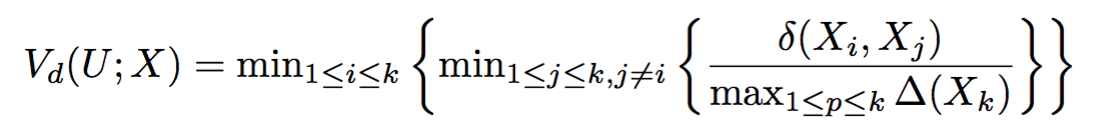
\includegraphics[scale=0.75]{dunnsindex}
	\caption{Formula  for Dunns Index}
	\label {fig:dunn}
	\end{figure}
\newpage
\item The indices obtained for the different K values are
\begin{verbatim}
Dunns index for k=2  = 0.260
Dunns index for k=3  = 0.037
Dunns index for k=4  = 0.023
Dunns index for k=5  = 0.031
Dunns index for k=6  = 0.031
Dunns index for k=7  = 0.031
Dunns index for k=8  = 0.023
Dunns index for k=9  = 0.031
Dunns index for k=10  = 0.031
\end{verbatim}

\item For Dunn's Index, the higher the better. For our data set, we obtain highest value for $K=2$. In other words, Our data is more suitable for 2 clusters. And using K=2 in K means algorithm should result in higher accuracy.
\end{enumerate}
\item \textbf{Davis-Bouldin Index}
\begin{enumerate}
\item We follow case 1 and seed the mean to zeros
\item Caclulate Davil-Bouldin Indices for K ranging from 2 to 10 for the V using the formula shown in figure \ref{fig:davis}
	\begin{figure}[h!]
	\centering
	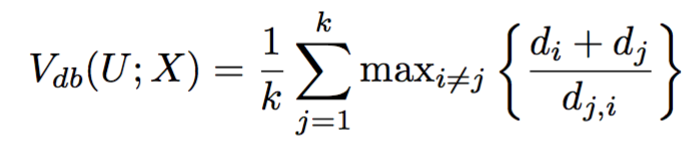
\includegraphics[scale=0.75]{Davis}
	\caption{Formula  for Davis-Bouldin Index}
	\label {fig:davis}
	\end{figure}
\item the values for the different values of K are
\begin{verbatim}
DaviesBouldin index for k=2  = 0.49
DaviesBouldin index for k=3  = 0.76
DaviesBouldin index for k=4  = 0.90
DaviesBouldin index for k=5  = 0.96
DaviesBouldin index for k=6  = 0.97
DaviesBouldin index for k=7  = 1.01
DaviesBouldin index for k=8  = 1.04
DaviesBouldin index for k=9  = 0.96
DaviesBouldin index for k=10  = 1.07
\end{verbatim}
\item For Davis-Bouldin Index, the lesser the better. The results shown above corresponds to the Dunn's Index. The Davis-Bouldin index for K=2 is the least hence, implies the same as the Dunn's index. If K=2 then the K means algorithm will give maximum performance.
\end{enumerate}

\begin{table}[]
\centering
\caption{Validity Index for mean = 0}
\label{my-label}
\begin{tabular}{lll}
K Value & Dunn's Index & Davies-Bouldin Index \\
\hline
\hline
2       & 0.260        & 0.49                 \\
3       & 0.037        & 0.76                 \\
4       & 0.023        & 0.90                 \\
5       & 0.031        & 0.96                 \\
6       & 0.031        & 0.97                 \\
7       & 0.031        & 1.01                 \\
8       & 0.023        & 1.04                 \\
9       & 0.031        & 0.96                 \\
10      & 0.031        & 1.07                \\
\hline
\end{tabular}
\end{table}


\end{enumerate}

\item \textbf{Dendrogram} A Dendrogram is a tree that represents the relationships or similarities among the samples in a group. 

\begin{enumerate}
\item We create a dendrogram with first 10 samples from each class(information taken from the labels in the dataset given). 
\item The first 10 are from species 1(1-10), 2nd 10 from second species(11-20), 3rd 10 from the third species(21-30) respectively.
\item The plot is available in the figure \ref{fig:dend1}
	\begin{figure}[h!]
	\centering
	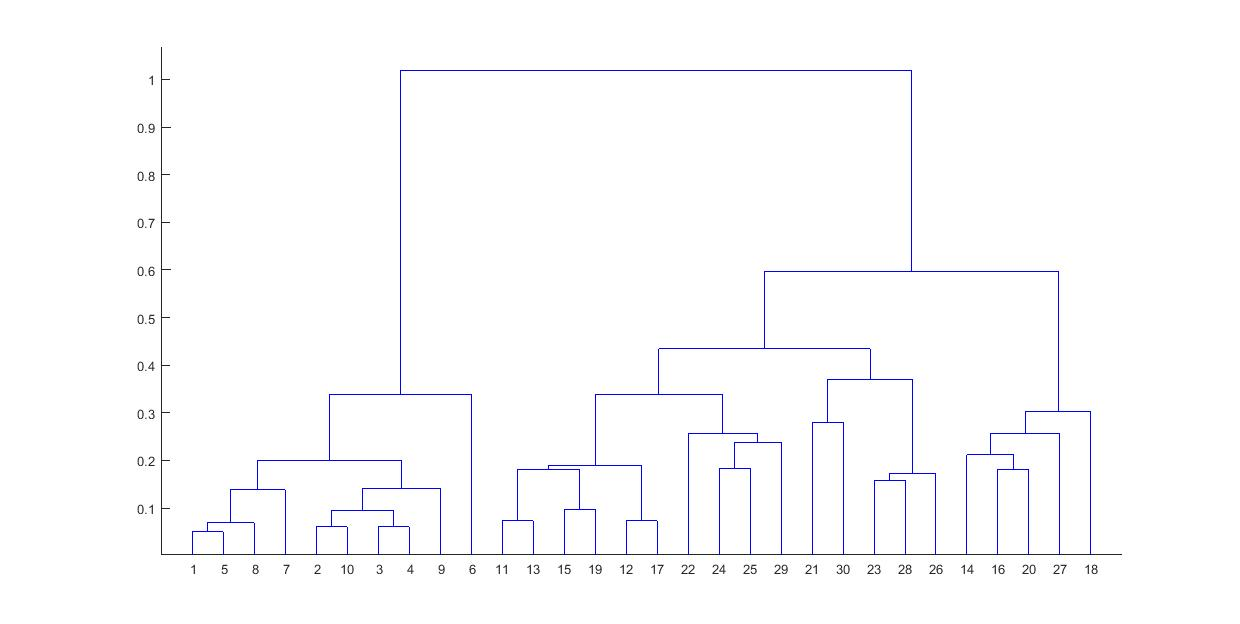
\includegraphics[scale=0.45]{Dendrogram}
	\caption{Dendrogram 1}
	\label{fig:dend1}
	\end{figure}
	\begin{figure}[h!]
	\centering
	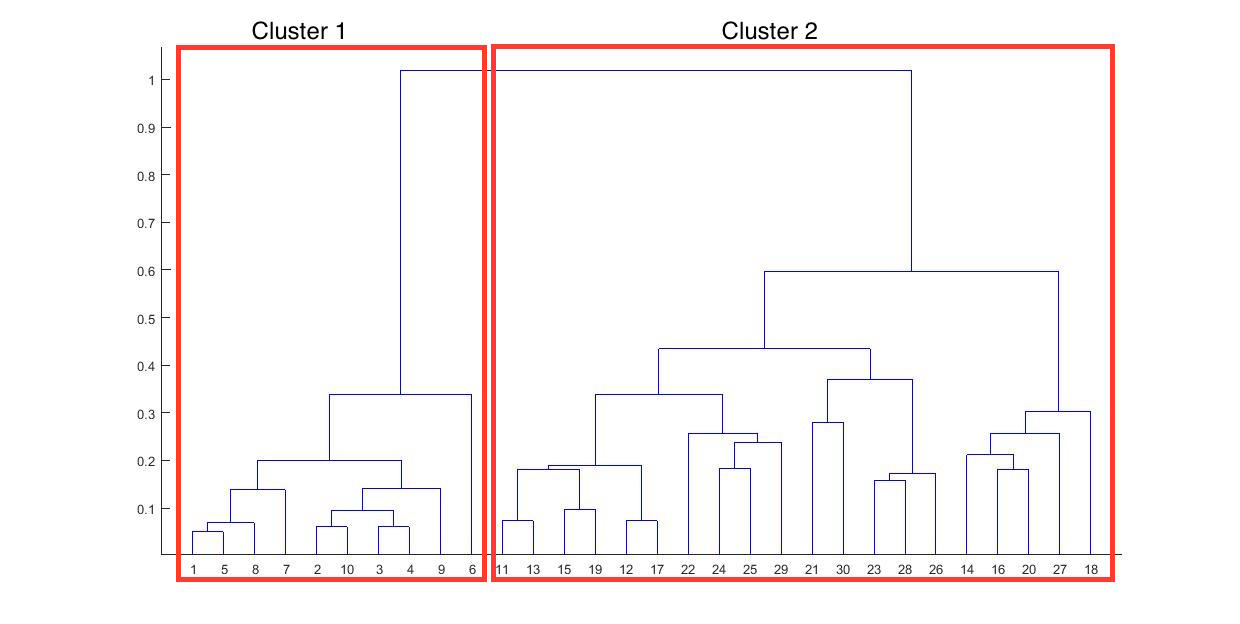
\includegraphics[scale=0.45]{Dendrogram_1}
	\caption{Dendrogram 2}
	\label{fig:dend2}
	\end{figure}
	\begin{figure}[h!]
	\centering
	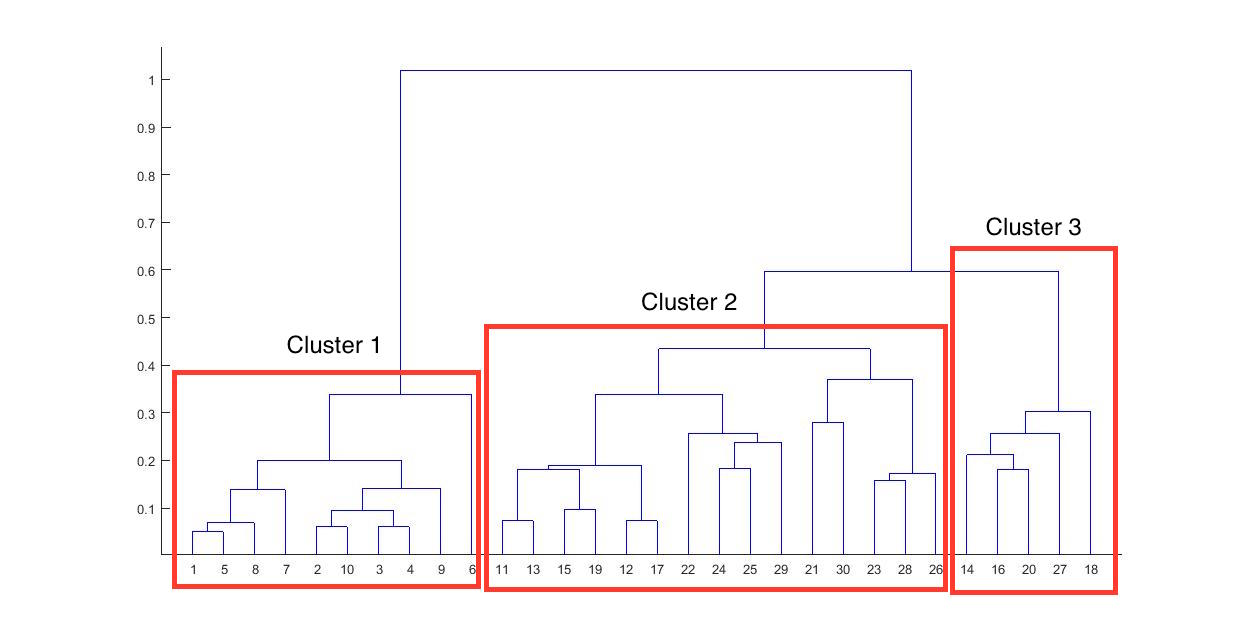
\includegraphics[scale=0.45]{Dendrogram_2}
	\caption{Dendrogram 3}
	\label{fig:dend3}
	\end{figure}
\item from the figure we can understand that the samples 20-30 are also similar to the species 2 and hence they are also classifies along with the class 2. This can be verified with the result from the K means algorithm.
\item From fig \ref{fig:dend2}, by clustering the data into 2 clusters the distance between the clusters measured in unweighted euclidean distance is large (approx ~0.3) hence, the distance between the centroids will me more in this case, hence K=2 will be a more better option for the given dataset.

\item From the figure \ref{fig:dend3} , by clustering the data into 3 clusters the distance between the clusters is lesser (approx ~0.1) hence this also proves that clustering the data into 2 clusters is more efficient. 
\end{enumerate}
\newpage
	
	\begin{figure}[h!]
	\centering
	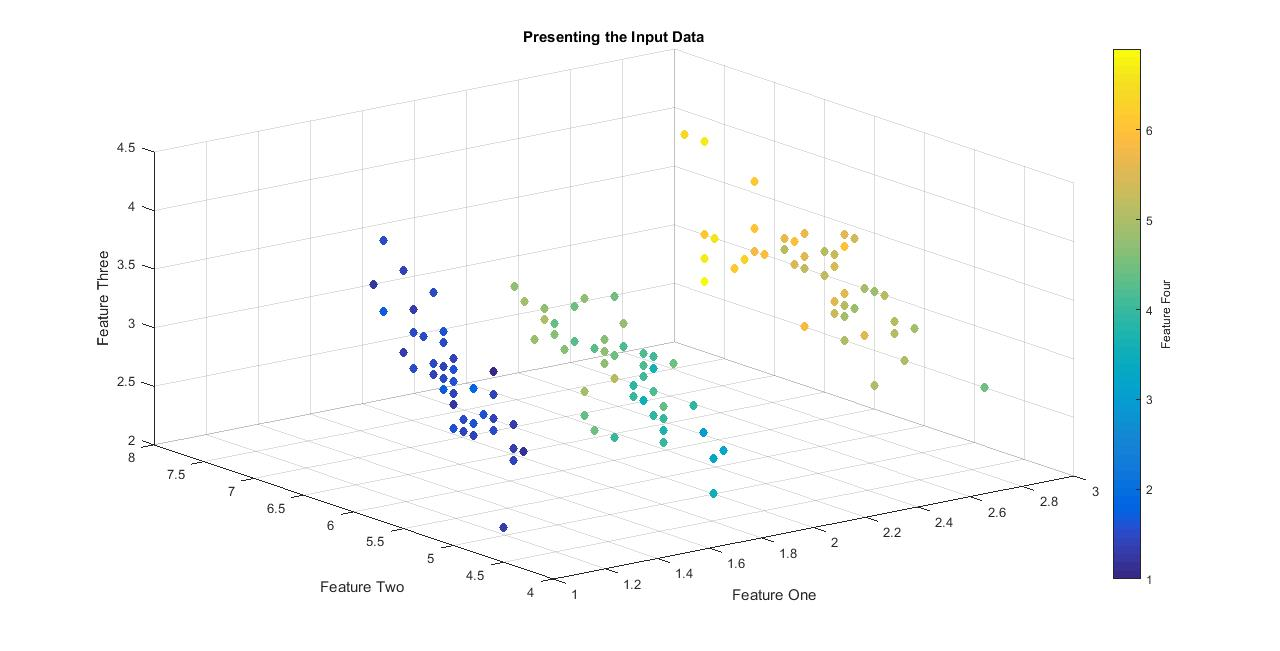
\includegraphics[scale=0.45]{DataPresentation}
	\caption{Presenting the Input Data}
	\label{fig:ipdata}
	\end{figure}
	\begin{figure}[h!]
	\centering
	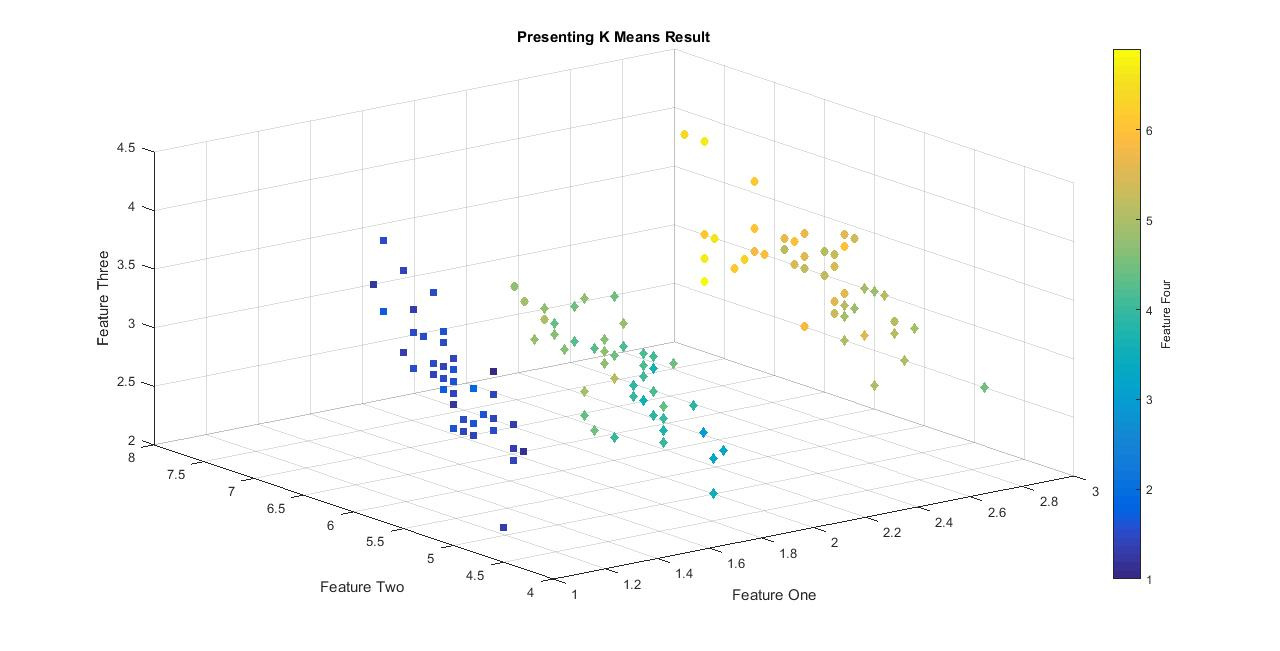
\includegraphics[scale=0.45]{PresentingKmeansResult}
	\caption{K means clustering when K = 3, Here Square is cluster 1, Diamond is cluster 2, Circles are cluster3}
	\label{fig:ClusterK3}
	\end{figure}
	\begin{figure}[h!]
	\centering
	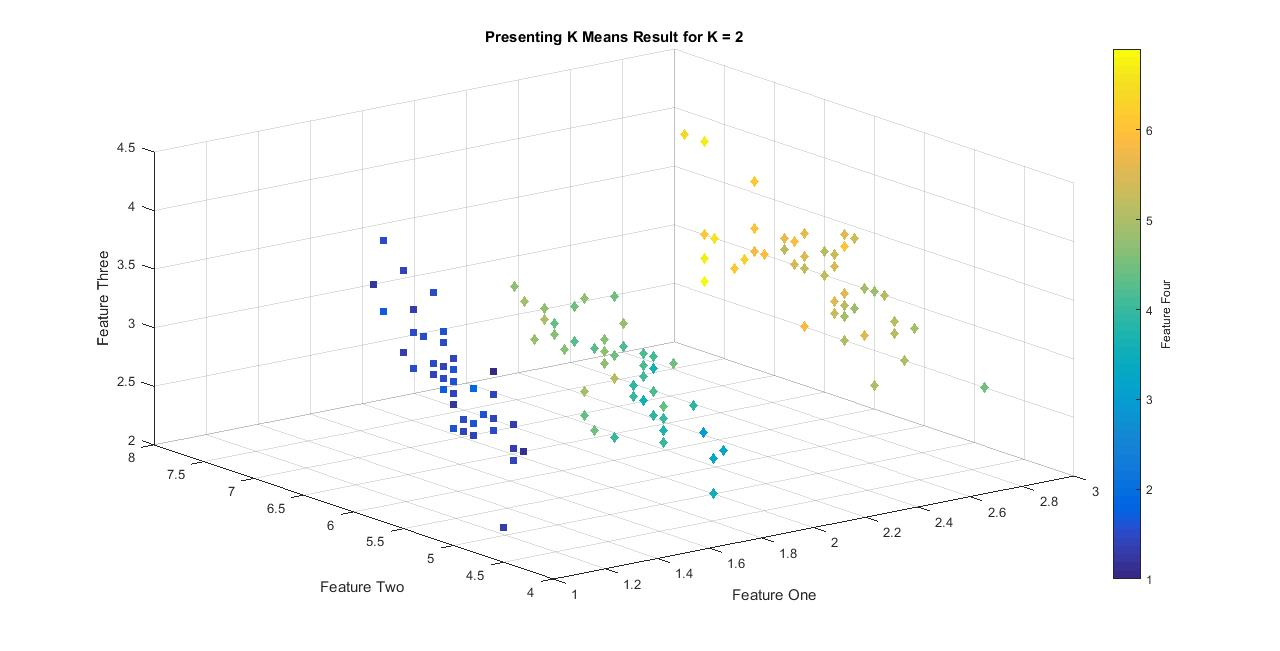
\includegraphics[scale=0.45]{PresentingKmeansResultforK2}
	\caption{K means clustering when K = 2, Here Squares are Cluster 1 \& Diamonds are Cluster 2 }
	\label{fig:ClusterK2}
	\end{figure}


\item \textbf{Observations}: The figure \ref{fig:ipdata} shows the input data in a projected space. From the image we can understand that the cluster 2 and cluster 3 have a lot of overlapping with respect to feature 4. In figure \ref{fig:ClusterK3} we can see that this feature 4 causes a lot of samples to be classified as another cluster. When we perform K means, for K =2  as shown in fig \ref{fig:ClusterK2} we can see that the data has been clustered into 2 clusters, with two species together forming one cluster. 




\end{enumerate}


\end{document}